\subsection{CU6 Eliminar Registro de Vehículo}
Esta pantalla es muy similar a la de Registrar Vehículo (figura \ref{fig:Pantalla Registrar Vehículo - Vista de Escenarios}) y a la de Modificar Vehículo (figura \ref{fig:Pantalla Modificar Registro de Vehículo - Vista de Escenarios}), sin embargo, esta pantalla esta diseñada para ser un 'mensaje de seguridad'. Muestra los datos que el usuario desea eliminar y al pulsar el botón 'Aceptar', el sistema ordena a la base de datos eliminar ese registro. Por otro lado, el botón 'Cancelar', cierra ese mensaje de seguridad y volvemos a la pantalla de Visualizar Agenda (figura \ref{fig:Pantalla Visualizar Agenda - Vista de Escenarios}).
\\
\begin{figure}[!h]
	\centering
	\includegraphics[width=1\textwidth]{./diseno/vescenarios/imagenes/eliminarVehículo}
	\caption{Pantalla Eliminar Registro de Vehículo - Vista de Escenarios}
	\label{fig:Pantalla Eliminar Registro de Vehículo - Vista de Escenarios}
\end{figure}
\\
Cuando se ha eliminado el registro de manera exitosa en la base de datos, el sistema mostrará una alerta (figura \ref{fig:Alerta4 - Vista de Escenarios}) como confirmación de que se ha borrado el registro de la base de datos.
\begin{figure}[!h]
	\centering
	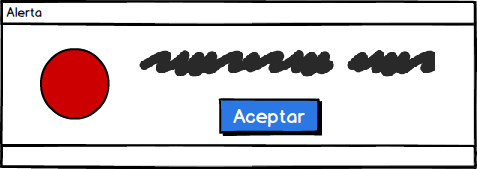
\includegraphics[width=0.5\textwidth]{./diseno/vescenarios/imagenes/alerta}
	\caption{Alerta Confirmación de Eliminación- Vista de Escenarios}
	\label{fig:Alerta4 - Vista de Escenarios}
\end{figure}